% EN.705.742 research paper, final version (RP3; the midpoint draft was RP2).
% Built on the course's IEEE conference template (conference_101719.tex).
% Build: bash paper/build.sh RP3   (latexmk + bibtex -> Ellis-RP3.pdf)
\documentclass[conference]{IEEEtran}
\IEEEoverridecommandlockouts
\usepackage{cite}
\usepackage{amsmath,amssymb,amsfonts}
\usepackage{graphicx}
\usepackage{textcomp}
\usepackage{xcolor}
\usepackage{booktabs}
\usepackage{url}
\DeclareMathOperator*{\softmax}{softmax}
\DeclareMathOperator*{\argmax}{arg\,max}
\DeclareMathOperator{\onehot}{onehot}
% \pending{} marks text not yet final.
\newcommand{\pending}[1]{\textcolor{gray!70!black}{\textit{[Final paper: #1]}}}

\begin{document}

\title{Interference-Aware Write Control for Bounded-Memory Recurrent Models\\
{\footnotesize Final paper}
\thanks{Research paper for EN.705.742 Advanced Applied Machine Learning,
Johns Hopkins University, Fall 2026. Midpoint draft submitted 2026-10-25;
this final version reports the full sweep.}
}

\author{\IEEEauthorblockN{Ryan Ellis}
\IEEEauthorblockA{\textit{Whiting School of Engineering} \\
\textit{Johns Hopkins University}\\
Baltimore, MD, USA \\
rellis26@jh.edu}
}

\maketitle

\begin{abstract}
Recurrent sequence models keep a fixed-size state, so when a sequence holds
more key-value associations than the state can carry, new writes degrade old
ones. Recent work adds a bounded memory beside the state with a rule for what
to admit, driven by input novelty, prediction residual, or position. This paper
asks whether a learned write controller that also measures \emph{interference},
the conflict between an incoming association and the ones already stored,
allocates a fixed slot budget better. We build a gated-linear-attention
backbone with a bounded slot memory, a learned controller with per-slot
interference features, two ablations of it, and four rule-based writers, all
sharing one backbone, budget, and data, and test them on multi-query
associative recall with key updates and distractors across 64 and 128
associations and 32, 64, and 128 slots, three seeds per cell, paired on
identical test sequences. Neither hypothesis holds. A parameter-free rule that admits every
key-value pair and nothing else beats every learned writer in every cell, by
6.6 points at 64 associations and 64 slots; the controller does beat the
proposal's own three baselines, by 20 to 63 points above 32 slots, but H1 is
defined against the strongest baseline and that is the rule. An ablation whose gate sees nothing derived from the stored memory
matches the controller's best ablation and beats the controller at both
decisive budgets, so the interference signal carries nothing a learned gate
can use here. Three findings explain why: the 32-slot cell is capacity-bound
for any writer (an ideal online writer caps at 43\%, any policy at 50\%); learned gates under-admit pairs,
which the admission statistics measure directly; and on a task whose queries
are uniform over keys, stored content cannot predict reuse, which the online
caching literature predicts. A pilot with skewed keys, where reuse is
predictable, shows the gate learns to reject distractors on two of three seeds and
still trails the rule. We provide the capacity-ceiling analysis and the pair-only reference as a
bar for learned admission policies.
\end{abstract}

\begin{IEEEkeywords}
linear attention, recurrent models, external memory, memory allocation,
associative recall, interference, gated linear attention
\end{IEEEkeywords}

%=====================================================================
\section{Introduction}
\label{sec:intro}

\subsection{The problem}

A Transformer remembers everything it has seen because its key-value cache grows
with the sequence~\cite{vaswani2017attention}. Recurrent alternatives, including
linear attention~\cite{katharopoulos2020linear}, gated linear
attention~\cite{yang2023gla}, DeltaNet~\cite{yang2024deltanet}, and selective
state space models~\cite{gu2023mamba}, replace the cache with a state of fixed
size. That makes inference cost constant per token, but it also makes memory a
scarce resource. When a sequence contains more associations than the state can
hold, a new write lands on directions already in use and the old association
degrades. Zoology~\cite{arora2023zoology} made this concrete with the multi-query
associative recall (MQAR) task, where recall accuracy of fixed-state models falls
off as the number of key-value pairs grows past the state's capacity. A recent
mechanistic study~\cite{lee2026howlinear} shows that the degradation tracks
\emph{memory load}, the number of overlapping associations stored, far more than
elapsed context.

Three 2026 papers attack this with explicit bounded memories beside the recurrent
state and a rule for what to write into them. HOLA~\cite{cui2026hola} keeps an
exact key-value cache and admits a token when the recurrent state's prediction
residual for it is large. Raven~\cite{afzal2026raven} keeps a fixed set of slots
and routes each token to a subset by a learned, input-dependent router.
Proteus~\cite{bayat2026proteus} activates memory capacity on a position schedule
so early tokens cannot pollute the whole memory. Each rule looks at the
\emph{input} (its novelty, its residual, its routing logits) or at
\emph{position}. None looks directly at the \emph{conflict} between the incoming
association and what is already stored. This paper tests whether that conflict
signal helps, under a controlled protocol fixed before the sweep, and finds that
it does not: on this task a learned writer that ignores the memory's contents
entirely matches or beats every other learned writer, and a parameter-free
rule beats them all.

\subsection{Research question and goals}

The research question is: \emph{at a fixed memory budget, does an explicit
per-slot interference estimate improve how a bounded memory is allocated,
measured as exact recall on associative recall tasks whose load exceeds the
budget?} The question is measurable (exact recall, paired against baselines on
identical test sequences), specific (one signal added to an otherwise shared
architecture), and relevant to a live gap in the literature
(Section~\ref{sec:related}).

The goal of the project is to answer it with a controlled architecture
comparison. The candidate solution is a small learned write controller that
receives, for every memory slot, the similarity of the incoming key to the slot's
key and the disagreement between the incoming value and the slot's value,
alongside input novelty and slot age. It outputs differentiable per-slot write
gates. Backbone, memory, and controller train jointly on query-answer
cross-entropy.

\subsection{Hypotheses}

\textbf{H1.} At matched total memory and training compute, the controller
improves exact recall by at least five percentage points over the strongest
validation-selected baseline on sequences with 64 to 128 distinct associations
at slot budgets of 32, 64, and 128. (The proposal named the 32-slot budget;
Section~\ref{sec:protocol} shows that cell is capacity-bound for every writer,
so the hypotheses are decided at 64 and 128 slots and the 32-slot column is
reported for completeness.)

\textbf{H2.} Removing the interference features while holding the controller's
size fixed reduces that gain, showing that the interference signal carries
information the input alone does not. (Tested against an ablation whose gate
sees nothing derived from the stored memory; Section~\ref{sec:controller}.)

\subsection{Approach and contributions}

The applied ML problem is supervised sequence-to-token prediction on a
synthetic recall task. The method of analysis is a controlled architecture
comparison: seven writers (the controller, two ablations of it, one modeled
on Raven's router, and four rule-based writers, two modeled on HOLA and
Proteus) on one
backbone, one memory, one data distribution, and one training schedule, with
three seeds per cell, paired bootstrap intervals over shared test sequences,
and explicit state-byte accounting. Every batch of runs after the proposal's
pilot was pre-registered with a prediction in a lab notebook before launch, and every change to the
protocol after the proposal is listed in Section~\ref{sec:changes}.
Everything is implemented in PyTorch; 108 sweep runs plus 60 follow-up runs
completed without a failure on one GPU.

The contributions are the answers and the tools that produced them:
\begin{enumerate}
\item \textbf{A negative result on both hypotheses, with the mechanism.}
A learned controller with interference features loses to a parameter-free
pair-only rule in all six cells (Table~\ref{tab:final}), and an ablation that
sees nothing from the memory beats the controller at both decisive budgets.
The gate statistics show why: the controller admits 69 to 82\% of pairs where
the rule admits all of them.
\item \textbf{A capacity ceiling for bounded-memory recall.} A simulation of
the ideal online writer gives the recall it can reach in a cell (43\% at 64
associations and 32 slots; 50\% for any policy, with perfect foreknowledge). It shows that the proposal's
target cell could not separate the hypotheses, and it is cheap enough to run
before any sweep.
\item \textbf{The pair-only rule as the reference.} Admit-every-pair-and-nothing-else is a reference every cited allocation
mechanism can be compared against: it
has no parameters, is 3 to 11~pp under the online ceiling, in part because it does
not overwrite updates in place, and here beats everything learned.
\item \textbf{A protocol lesson.} Hyperparameters selected on one seed, in a
capacity-bound cell, produced a false positive for H2 that only an
equal-learning-rate check exposed; the paper reports both comparisons and the
re-selection that confirmed the controller's setting.
\end{enumerate}

Section~\ref{sec:related} surveys allocation mechanisms, Section~\ref{sec:method}
gives the task, architecture, controller, and baselines,
Section~\ref{sec:results} the protocol, the sweep, the follow-up checks, and
the pilot that validated the pipeline, Section~\ref{sec:discussion} the
interpretation, including the online-caching view and the limitations, and
Section~\ref{sec:conclusion} what the study rules out and what it does not.

%=====================================================================
\section{Related Work}
\label{sec:related}

\subsection{Survey method}

Following the PRISMA 2009 structure~\cite{moher2009prisma} in a light form suited
to a course paper: a stated question, explicit eligibility criteria, documented
searches, and a flow count. The question was \emph{which mechanisms decide what
a bounded-memory sequence model writes, and has interference between stored
associations been used as a write signal?} Three arXiv searches on 2026-10-15,
the proposal's references, and eleven foundational papers identified 44
records, and citation chasing from the included papers on 2026-10-24 added
2 more; 33 were unique; 9 were screened out by title and abstract (retrieval
augmentation, agent memory, video, serving systems, surveys); 24 were assessed
and included. The full log with queries and per-record exclusion reasons is in
the project repository (\texttt{paper/prisma/search-log.md}).

\subsection{Bounded-state backbones and their write rules}

Linear attention~\cite{katharopoulos2020linear} stores associations as a sum of
outer products $\sum_t v_t k_t^\top$; every token writes with equal weight.
Fast-weight programmers~\cite{schlag2021fastweight} introduced the delta rule,
which subtracts the state's current prediction before adding, so a write
\emph{corrects} rather than accumulates. GLA~\cite{yang2023gla} adds a
data-dependent decay gate; DeltaNet~\cite{yang2024deltanet} and Gated
DeltaNet~\cite{yang2024gateddeltanet} make the delta rule and its decay trainable
at scale; Mamba~\cite{gu2023mamba} reaches a similar place through selective
state-space parameters. Based~\cite{arora2024based} combines a small
linear-attention state with sliding-window attention and shows the
recall-throughput trade-off directly. ABC~\cite{peng2021abc} frames linear
attention and several of its relatives as attention over a bounded memory of
fixed size, with a \emph{control} function that decides how each token is
organized into the memory, and replaces the heuristic control of earlier
variants with one learned from context. Gated Slot Attention~\cite{zhang2024gsa}
builds on ABC, and its successor GSA-2~\cite{li2026gsa2} organizes the state as
shared latent slots with decoupled erase and write gates on both the key and
value side.
Variational Linear Attention~\cite{pandey2026vla} casts each write as a
regularized least-squares step and bounds the state norm. In all of these the
write decision is a function of the token and a learned gate; the state is
addressed implicitly through key overlap, and the mechanistic study by Lee et
al.~\cite{lee2026howlinear} shows that recall degrades with the number of
overlapping writes.

\subsection{Allocation, routing, and eviction into explicit memory}

Neural Turing Machines~\cite{graves2014ntm} and the Differentiable Neural
Computer~\cite{graves2016dnc} are the classical learned-allocation designs: NTM
addresses by content and location, DNC adds a usage vector and allocates the
least-used slot. Our age and usage features are DNC-style; our interference
features are not in either model. Titans~\cite{behrouz2024titans} gates memory
updates by \emph{surprise}, the gradient of a reconstruction loss, which is an
input-side novelty signal. HOLA~\cite{cui2026hola} admits tokens to an exact
cache when the delta-rule residual is large, again a property of the token
against the state's prediction rather than a per-slot conflict.
Raven~\cite{afzal2026raven} learns an input-dependent router over a fixed slot
set. ARM~\cite{zeng2026arm} does the same for a Transformer KV cache with a
Gumbel-softmax router and sigmoid-gated blends. IndexMem~\cite{yang2026indexmem}
trains an indexer to score KV entries for eviction. Fast-weight Product Key
Memory~\cite{zhao2026fwpkm} updates only activated slots of a large sparse
memory. RAM-Net~\cite{xiao2026ramnet} is the closest in motivation to this
paper: it names the mixing of unrelated tokens in a shared state as the cause
of poor fine-grained recall and answers it with an address decoder that maps
each key to a sparse set of slots, so tokens with disjoint addresses cannot
interfere. The address is a function of the key alone; the decoder never
inspects what a slot currently holds. Proteus~\cite{bayat2026proteus} sidesteps allocation by unlocking
capacity on a position schedule, and Memory Caching~\cite{behrouz2026memcache}
sidesteps it by letting memory grow. Zoology~\cite{arora2023zoology} and
RULER~\cite{hsieh2024ruler} supply the recall evaluations the field uses.

\subsection{The gap}

Every allocation rule above conditions on the input (novelty, surprise,
residual, router logits, a key's address) or on position (schedule, recency,
usage). ABC and RAM-Net come nearest, since both learn a per-token slot
assignment and RAM-Net states interference as its target, but each decides
from the token alone and avoids conflict by construction rather than measuring
it. None computes, for each candidate slot, whether the incoming association
conflicts with the one stored there, even though the capacity analyses say
that this conflict is what limits recall. The controller in Section~\ref{sec:controller}
adds exactly that signal and nothing else, so the comparison isolates its value.

%=====================================================================
\section{Methodology}
\label{sec:method}

\subsection{Task: multi-query associative recall with updates and distractors}
\label{sec:task}

Each sequence has three regions (Fig.~\ref{fig:block}). The \emph{context
block} holds $N$ queried pairs and $D$ distractor pairs, each a key token
followed by a value token, in random order. The \emph{update block} repeats $U$
of the queried keys with a new value; the correct answer for an updated key is
its latest value. The \emph{query region} presents each queried key once more;
the label at that position is the final value. Query positions follow Zoology's
power-law gap distribution, shifted by a minimum delay $\delta$ so delay is a
separate knob. The vocabulary is split into key tokens and value tokens. Loss and
metrics use only the $N$ answer positions per sequence. The generator is adapted
from Zoology's \texttt{multiquery\_ar} and \texttt{forgetting\_mqar} (Apache-2.0)
with the distractor and delay extensions added.

Pilot setting: vocabulary 2048, sequence length 128, $N = 16$, $U = 4$, $D =
4$, $\delta = 0$, so 24 associations compete for $S = 16$ slots. This is smaller
than the proposal's 64-association, 32-slot target; Section~\ref{sec:pilot}
reports what happened at the target and why the pilot moved. Splits: 100{,}000
train, 5{,}000 validation, 10{,}000 test, generated from distinct seeds with
exact-duplicate sequences removed from validation and test.

\begin{figure*}[t]
\centering
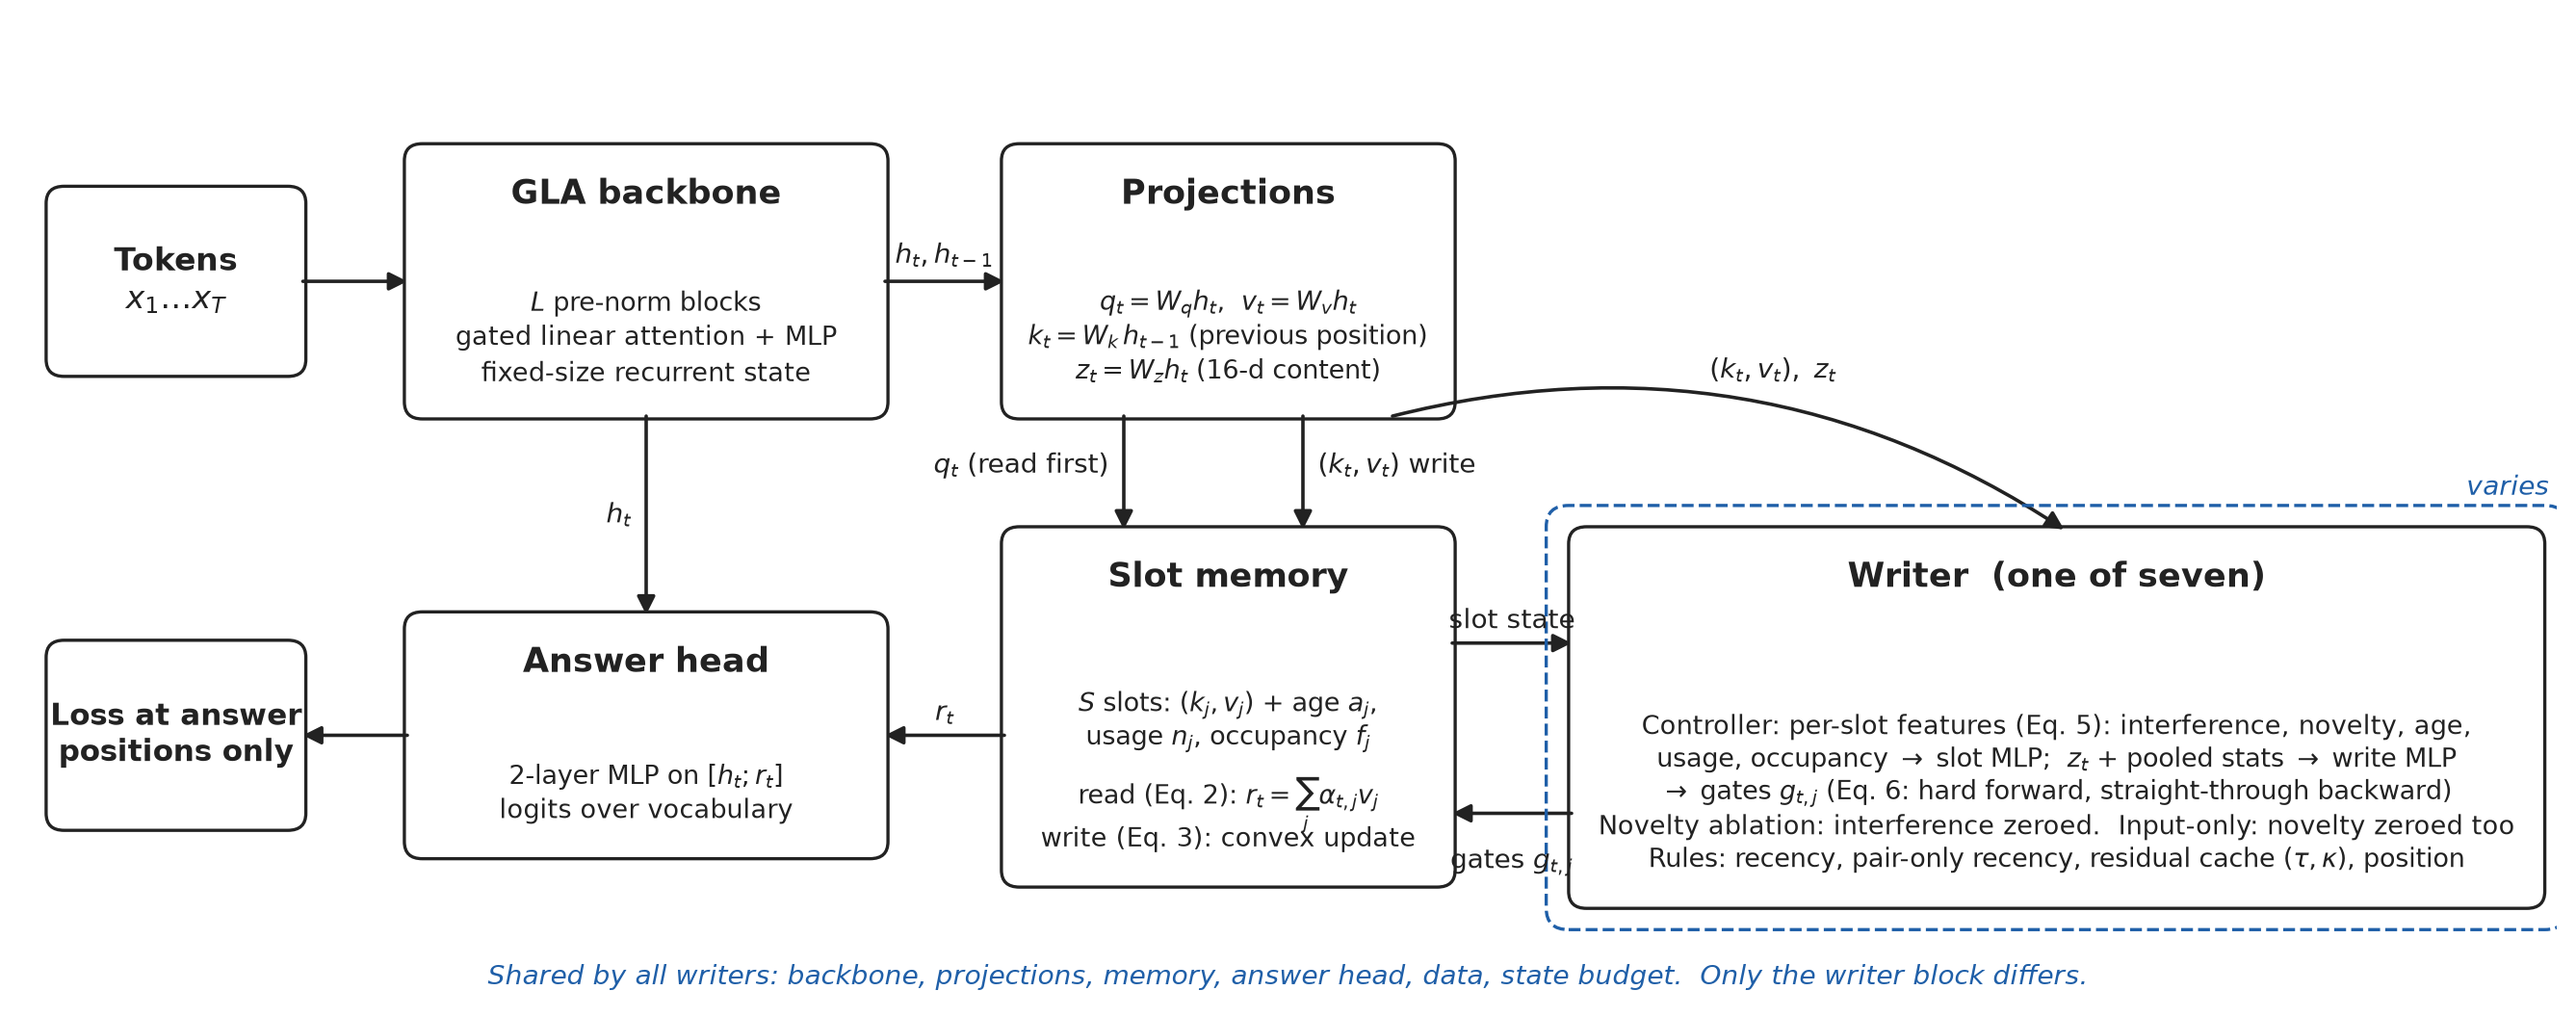
\includegraphics[width=\textwidth]{figures/block-diagram.png}
\caption{System block diagram at one position $t$. The GLA backbone output
$h_t$ is projected to a query $q_t$ and value $v_t$; the key $k_t$ is projected
from the previous position's output $h_{t-1}$ (Section~\ref{sec:arch}). The
slot memory is read with $q_t$ \emph{before} it is written. The writer compares
the incoming pair $(k_t, v_t)$ with every slot to form the per-slot features of
Eq.~\eqref{eq:features} (the novelty ablation zeroes the two interference
features; the input-only ablation also zeroes novelty)
and emits the gates $g_{t,j}$ of Eq.~\eqref{eq:gate}; the fixed baselines
replace this block with their rule (Table~\ref{tab:baselines}). The convex
update of Eq.~\eqref{eq:write} writes the memory, and the answer head sees
$[h_t; r_t]$. Loss is taken at answer positions only.}
\label{fig:block}
\end{figure*}

\subsection{Architecture}
\label{sec:arch}

\subsubsection{Backbone}
$L$ pre-norm blocks of gated linear attention (GLA)~\cite{yang2023gla} with an
MLP, using the \texttt{flash-linear-attention} PyTorch implementation. GLA keeps,
per head and layer, a $d_k \times d_v$ recurrent state with a learned
data-dependent decay. Pilot: $L = 2$, $d_{\text{model}} = 256$, 4 heads,
2048-token vocabulary. The sweep uses the same two-layer model with an
8192-token vocabulary (5.99M parameters); the proposal's 20M-parameter scale
was not reached.

\subsubsection{Projections}
From the backbone output $h_t \in \mathbb{R}^{d_{\text{model}}}$: $q_t = W_q
h_t$, $v_t = W_v h_t$, and $k_t = W_k h_{t-1}$, all in $\mathbb{R}^{d}$ with $d
= 128$. The key is projected from the \emph{preceding} position because an
association is a (key, value) token pair: the value token's own representation
carries the value, and the token before it carries the key. Without this
one-step shift the backbone must first learn to copy each key one position
forward before the memory can store anything retrievable; in a pilot diagnostic
that cost a four-fold difference in recall at equal training steps
(Section~\ref{sec:pilot}). All writers share this projection, so it does not
favor the controller.

\subsubsection{Slot memory}
$S$ slots, each a key $k_j$ and value $v_j$ in $\mathbb{R}^{d}$, plus scalar
age $a_j$, usage $c_j$, and occupancy $f_j$. Read is attention over occupied
slots:
\begin{equation}
\alpha_{t,j} = \softmax_j\!\left(\frac{q_t^\top k_j}{\sqrt{d}} + \log f_j\right),
\qquad r_t = \sum_j \alpha_{t,j} v_j .
\end{equation}
Write is a convex update of every slot, as in the proposal:
\begin{equation}
m_{t,j} = (1 - g_{t,j})\, m_{t-1,j} + g_{t,j}\, u_t,
\label{eq:write}
\end{equation}
where $m_j = (k_j, v_j)$ is the slot's contents and $u_t = (k_t, v_t)$ the
incoming association,
with $a_j \leftarrow (a_j + 1)(1 - g_{t,j})$, $c_j \leftarrow c_j + g_{t,j}$,
and $f_j \leftarrow (1 - g_{t,j}) f_j + g_{t,j}$. At each position the memory is
read \emph{before} it is written, so a query token sees what was stored before
it.

\subsubsection{Answer head}
A two-layer MLP on $[h_t ; r_t]$ produces logits over the vocabulary.
Cross-entropy is computed at answer positions only.

\subsection{The interference-aware controller}
\label{sec:controller}

For each slot $j$ the controller builds a six-dimensional feature vector
\begin{equation}
\begin{split}
\phi_{t,j} = \Big[\,
&\underbrace{\cos(k_t, k_j),\; \tfrac{1}{\sqrt{d}}\lVert v_t - v_j \rVert}_{\text{interference}},\\
&\underbrace{1 - \max_{j'} \cos(k_t, k_{j'})}_{\text{novelty}},\;
\tfrac{a_j}{T},\; \tfrac{c_j}{T},\; f_j \,\Big],
\end{split}
\label{eq:features}
\end{equation}
where $T$ is the sequence length. The first feature is high when the incoming
key would land on a slot that already holds a similar key, which is the
condition under which a write \emph{overwrites} rather than \emph{adds}. The
second says whether that overwrite would change the stored answer. Together they
distinguish a harmless duplicate (similar key, same value) from a genuine key
update (similar key, new value) and from a collision between unrelated
associations whose keys happen to be close.

A two-layer MLP maps $\phi_{t,j}$ to a logit $\ell_{t,j}$: this decides
\emph{where} a write goes, from interference and slot age alone. A second small
MLP decides \emph{whether} to write at all, producing a scalar logit $w_t$ from
a pooled memory summary (novelty, mean occupancy, mean value disagreement)
concatenated with $c_t = W_c h_t \in \mathbb{R}^{16}$, a low-dimensional
projection of the current token's representation. The content input is what
lets the controller learn that a value token following a key is worth storing
and a filler token is not; without it, the decision to write could depend only
on memory statistics, and in the pilot diagnostics learning then depended on
luck (Section~\ref{sec:pilot}). A learnable scalar prior $\beta$ (initialized to
5) adds $\beta\,(a_j/T + 1 - f_j)$ to $\ell_{t,j}$, so at initialization the
controller prefers empty and then oldest slots, which is the recency writer; the
MLP only has to learn deviations from it. The gate is
\begin{equation}
g_{t,j} = \sigma(w_t)\, \onehot\!\big(\argmax_j \ell_{t,j}\big),
\label{eq:gate}
\end{equation}
with the straight-through estimator: the forward pass writes exactly one slot,
and the backward pass uses the gradient of $\softmax_j(\ell_{t,j})$ in its
place. The write can still be suppressed entirely through $\sigma(w_t)$. A fully
soft gate was tried first and did not learn: at initialization it spreads each
association across all slots, the memory never holds a retrievable entry, and
so no gradient arrives to sharpen it. Hard forward selection with a soft
backward path is the same device ARM uses for its slot router~\cite{zeng2026arm}.
The controller has 1{,}859 parameters in the pilot (including the prior), plus
4{,}112 in the content projection; the full two-layer pilot model has 2.84M. Its
decision depends only on the current association and the memory, so it adds no
per-sequence state beyond the memory's own age, usage, and occupancy scalars,
which are counted in the budget.

\textbf{H2 ablations.} Setting \texttt{interference=False} zeroes the two
per-slot interference features and leaves everything else identical, including
parameter count. It keeps the novelty feature, which is itself derived from the
stored keys (one minus the maximum key similarity), so this \emph{novelty
ablation} is a router that sees whether the incoming key is already in memory
but not where or with what value; it is the simplified form of Raven's routing
signal. A second ablation, \texttt{novelty=False} as well, is the
\emph{input-only ablation}: its gate sees only the content projection of the
current token and the slots' age, usage and occupancy, nothing derived from
stored keys or values. H2 as stated is the comparison against the input-only
ablation; the novelty ablation separates the per-slot detail from the global
signal.

\subsection{Baselines}
\label{sec:baselines}

All writers share the backbone, projections, memory, and answer head; only the
gate rule differs (Table~\ref{tab:baselines}). Each is a deliberate
simplification of the cited mechanism, re-implemented from the paper's
description because none of the three has public code at the time of writing.

\begin{table}[t]
\caption{Writers compared. All share the backbone, projections, memory, and
answer head.}
\label{tab:baselines}
\centering
\footnotesize
\begin{tabular}{@{}p{0.23\columnwidth}p{0.50\columnwidth}p{0.17\columnwidth}@{}}
\toprule
Writer & Gate rule & Models \\
\midrule
Interference controller & Eq.~\eqref{eq:gate} on the six features of Eq.~\eqref{eq:features} & proposed \\
Recency & $g_{t,j} = 1$ for the oldest (or first empty) slot, else 0, at every position & trivial control \\
Pair-only recency & recency gate applied only at the value position of a pair (uses the task layout) & rule-based reference \\
Novelty ablation & controller with the two per-slot interference features zeroed (keeps key novelty) & Raven~\cite{afzal2026raven} \\
Input-only ablation & controller with all stored-content features zeroed (content projection, age, usage, occupancy only) & H2 as stated \\
Residual cache & write to the oldest slot with gate $\sigma(\beta(\lVert r_t(k_t) - v_t\rVert/\sqrt{d} - \tau))$, learned $\tau, \beta$ & HOLA~\cite{cui2026hola} \\
Position activation & slot $j$ unlocked at position $\lceil jT/S \rceil$; recency among unlocked slots & Proteus~\cite{bayat2026proteus} \\
\bottomrule
\end{tabular}
\end{table}

\subsection{Training, accounting, and implementation}
\label{sec:training}

AdamW ($\beta = (0.9, 0.95)$, weight decay 0.1 on matrices), linear warmup then
cosine decay, gradient clipping at 1.0, bf16 autocast for the backbone with the
memory loop in fp32. Hyperparameters (learning rate, controller hidden size) are tuned on
validation only. The pilot used learning rate $3 \times 10^{-4}$ (chosen over
$10^{-3}$ on validation, Section~\ref{sec:pilot}), controller hidden size 64,
batch 64, 200 warmup steps, and 4{,}000 steps. State bytes per sequence are
reported as backbone recurrent state plus $S(2d + 3)$ floats of memory plus any
writer statistics; for the two-layer pilot model that is 64~KB backbone, 16~KB
memory, 0 writer, 80~KB in all, identical across writers.

The model, data generator, training loop, metrics, and experiment scripts are
written in PyTorch and live in the project repository with unit tests
(\texttt{pytest}) covering the data splits, the memory update, the gates, and
gradient flow. One command runs one (writer, seed, config) cell and writes a
results file; an aggregation script computes the tables and paired bootstrap
intervals reported below. A companion notebook
(\texttt{Ellis-RP2-prototype.ipynb}) walks through the generator, the model,
a short training run, and the statistics on sample data.

%=====================================================================
\section{Experiments and Results}
\label{sec:results}

\subsection{Experimental protocol}
\label{sec:protocol}

\textit{Factors.} Memory budget $S \in \{32, 64, 128\}$; associations $N \in
\{64, 128\}$; writer $\in$ \{controller, novelty ablation, recency, pair-only
recency, residual, position\} plus the input-only ablation in the follow-up. Updates and distractors fixed at $N/4$ each; a delay
sweep at $N = 64$ was planned and not run. The $N = 64$ column trains at length 512 and tests
at 512, 1024, and 2048; the $N = 128$ column trains at length 1024 and tests at
1024, 2048, and 4096, because its context block plus queries ($2 \cdot 192 + 128$
tokens) does not fit in 512. Test sequences are freshly generated.

\textit{Capacity ceiling.} A writer that cannot see the future can at best admit
every pair, overwrite updated keys in place, and evict the oldest pair when
full. Simulated on the generator, this pair-only policy reaches 43\% exact
recall at $N = 64$, $S = 32$ (50\% with perfect foreknowledge of which pairs
will be queried), 81\% at $S = 64$ (100\% with foreknowledge), and 100\% at
$S = 128$. The $S = 32$ cell is therefore capacity-bound: the whole margin that
allocation can win there is 7 points, and the hypotheses are decided at
$S = 64$, where rejecting distractors is worth 19 points. The pair-only recency
baseline implements exactly this ceiling policy, so it is the reference against
which learned allocation must be judged; naive recency, which writes at every
position, holds only the last $S$ tokens and sits at chance at these densities.

\textit{Checkpoint selection.} Each run is evaluated at the checkpoint with the
best validation recall during training (validation is 1{,}280 held-out
sequences scored every 500 steps), not at the last step, and the selected step
is reported. On this task the cosine tail can move a run from the pair-only
write policy into a worse one (Section~\ref{sec:pilot}); best-validation
selection reports the policy a run reached, and is how the reference MQAR
work reports accuracy~\cite{arora2023zoology}.

\textit{Seeds and statistics.} Three seeds per cell. Primary metric is exact
recall: the fraction of answer positions predicted exactly, averaged over the
10{,}000 test sequences. Each cell reports mean over seeds and a 95\% bootstrap
confidence interval over test sequences~\cite{efron1979bootstrap}; H1 is tested
with a \emph{paired} bootstrap on the per-sequence difference between the
controller and the best baseline, since all writers see the same test
sequences. Secondary metrics: recall by association density ($N/S$), state
bytes, training and evaluation throughput, and the write-gate statistics (mean
gate mass, slot entropy) that show \emph{how} each writer uses its budget.

\textit{Selection.} The learning rate for each writer and the controller's
hidden size are chosen on validation recall at $N = 64$, $S = 32$ and then
frozen.

\subsection{Results for H1 and H2}
\label{sec:final-results}

Table~\ref{tab:final} is the primary result: exact recall for every writer at
every budget and load, mean over three seeds, 108 runs with no failures.
Fig.~\ref{fig:sweep} shows the $N = 64$ column, its length generalization, and
the admission statistics behind it; Fig.~\ref{fig:sweep128} the same for
$N = 128$.

\begin{table*}[t]
\caption{Primary result. Exact recall (\%) at the training length (512 for
$N = 64$, 1024 for $N = 128$), mean $\pm$ standard deviation over three seeds on
10{,}000 test sequences; updates and distractors at $N/4$; best-validation
checkpoint. Bottom rows: mean paired difference in percentage points over test
sequences pooled across seeds, with the three per-seed differences in
parentheses. The pooled 95\% bootstrap interval is within $\pm 0.3$~pp of
the mean in every cell (it reflects test-sequence sampling only), so a cell is
decided by the sign agreement of the seeds; where they disagree the cell is
undecided. The last block is the equal-learning-rate H2 check: the ablation
trained at the controller's rate, and the paired differences with both writers
at the same rate (the sweep rows above compare each writer at its own
validation-selected rate). Generated by
\texttt{experiments/analysis/sweep\_paper.py}.}
\label{tab:final}
\centering
\scriptsize
\setlength{\tabcolsep}{3pt}
\begin{tabular}{@{}lcccccc@{}}
\toprule
 & \multicolumn{3}{c}{$N = 64$ associations} & \multicolumn{3}{c}{$N = 128$ associations} \\
\cmidrule(lr){2-4}\cmidrule(lr){5-7}
Writer & $S{=}32$ & $S{=}64$ & $S{=}128$ & $S{=}32$ & $S{=}64$ & $S{=}128$ \\
\midrule
Controller & 22.9 {\scriptsize$\pm$5.5} & 63.5 {\scriptsize$\pm$0.6} & 66.8 {\scriptsize$\pm$13.5} & 6.5 {\scriptsize$\pm$4.6} & 23.7 {\scriptsize$\pm$6.2} & 39.8 {\scriptsize$\pm$10.5} \\
Novelty ablation & 27.7 {\scriptsize$\pm$3.3} & 45.6 {\scriptsize$\pm$8.1} & 77.3 {\scriptsize$\pm$11.0} & 10.8 {\scriptsize$\pm$7.6} & 31.8 {\scriptsize$\pm$0.6} & 61.7 {\scriptsize$\pm$2.4} \\
Pair-only recency & 40.1 {\scriptsize$\pm$0.0} & 70.1 {\scriptsize$\pm$0.0} & 100.0 {\scriptsize$\pm$0.0} & 25.1 {\scriptsize$\pm$0.0} & 40.0 {\scriptsize$\pm$0.0} & 70.0 {\scriptsize$\pm$0.0} \\
Recency & 0.0 {\scriptsize$\pm$0.0} & 0.0 {\scriptsize$\pm$0.0} & 29.0 {\scriptsize$\pm$0.0} & 0.0 {\scriptsize$\pm$0.0} & 0.0 {\scriptsize$\pm$0.0} & 0.0 {\scriptsize$\pm$0.0} \\
Residual cache & 30.2 {\scriptsize$\pm$10.3} & 0.2 {\scriptsize$\pm$0.3} & 0.0 {\scriptsize$\pm$0.0} & 5.3 {\scriptsize$\pm$7.5} & 3.5 {\scriptsize$\pm$4.9} & 0.1 {\scriptsize$\pm$0.1} \\
Position activation & 0.0 {\scriptsize$\pm$0.0} & 0.0 {\scriptsize$\pm$0.0} & 0.0 {\scriptsize$\pm$0.0} & 0.0 {\scriptsize$\pm$0.0} & 0.0 {\scriptsize$\pm$0.0} & 0.0 {\scriptsize$\pm$0.0} \\
\midrule
H1: ctrl $-$ best rule-based (pp) & -17.2 {\scriptsize(-21, -21, -9)} & -6.6 {\scriptsize(-6, -6, -7)} & -33.2 {\scriptsize(-52, -25, -22)} & -18.6 {\scriptsize(-25, -16, -15)} & -16.3 {\scriptsize(-8, -21, -20)} & -30.2 {\scriptsize(-15, -39, -36)} \\
H2: ctrl $-$ novelty ablation (pp) & -4.8 {\scriptsize(-7, -6, -2)} & +17.9 {\scriptsize(+7, +25, +23)} & -10.5 {\scriptsize(-45, +6, +8)} & -4.3 {\scriptsize(+0, -7, -6)} & -8.1 {\scriptsize(+1, -14, -12)} & -21.8 {\scriptsize(-8, -27, -30)} \\
\midrule
Novelty ablation at $3\times10^{-4}$ & -- & 65.8 {\scriptsize$\pm$0.4} & 96.0 {\scriptsize$\pm$0.2} & -- & -- & -- \\
H2, both at $3\times10^{-4}$ (pp) & -- & -2.3 {\scriptsize(-3, -1, -3)} & -29.2 {\scriptsize(-49, -21, -18)} & -- & -- & -- \\
H2, both at $10^{-3}$ (pp) & -- & -4.1 {\scriptsize(-7, -5, +1)} & -6.2 {\scriptsize(-22, -3, +7)} & -- & -- & -- \\
Input-only ablation at $3\times10^{-4}$ & -- & 66.0 {\scriptsize$\pm$0.1} & 94.0 {\scriptsize$\pm$1.2} & -- & -- & -- \\
Input-only $-$ controller at $3\times10^{-4}$ (pp) & -- & +2.5 {\scriptsize(+2, +2, +3)} & +27.2 {\scriptsize(+46, +21, +15)} & -- & -- & -- \\
\bottomrule
\end{tabular}
\end{table*}

\begin{figure*}[t]
\centering
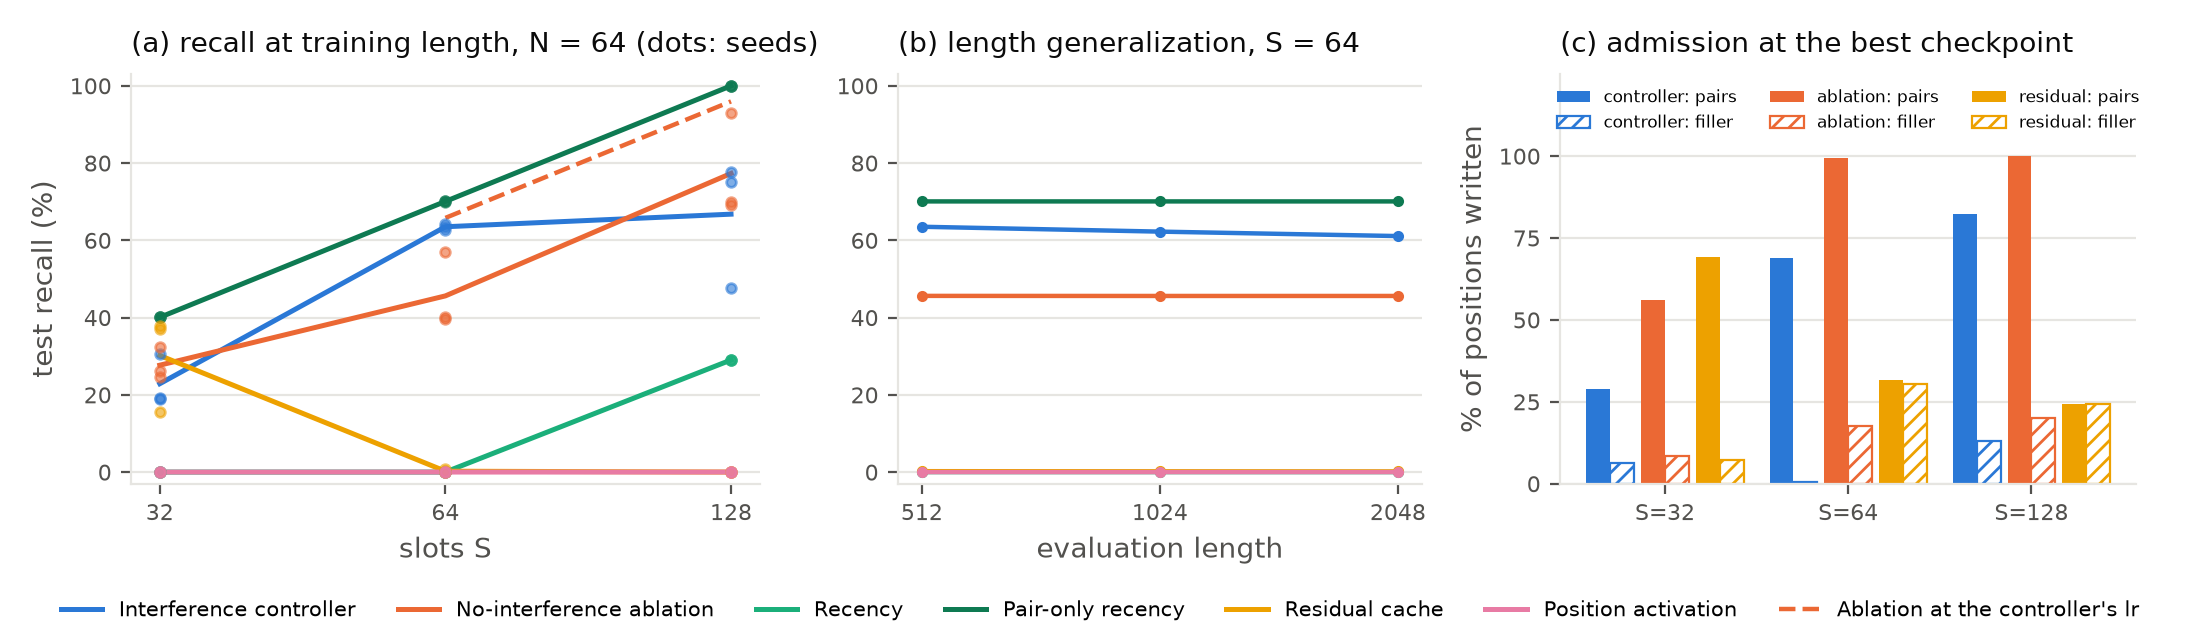
\includegraphics[width=\textwidth]{figures/sweep.png}
\caption{The $N = 64$ column of the sweep. (a) Test recall at the training
length against slot budget, mean over three seeds (lines) and each seed
(dots). Pair-only recency, which has no parameters in the writer, is above the
controller at every budget; the dashed line is the novelty ablation retrained at the
controller's learning rate (the equal-rate H2 check) and the dotted line the
input-only ablation at that rate. (b) Recall against evaluation length at $S = 64$:
flat for every writer except the controller, which loses 2.4~pp from 512 to
2048. (c) Admission at the best checkpoint: fraction of key-value pairs
written (solid) and of filler tokens written (hatched). The controller admits
69\% of pairs at $S = 64$ and 82\% at $S = 128$; the ablation admits every
pair but also 18--20\% of filler; the residual cache above $S = 32$ writes a
quarter to a third of every token class, i.e.\ it does not discriminate.}
\label{fig:sweep}
\end{figure*}

\begin{figure*}[t]
\centering
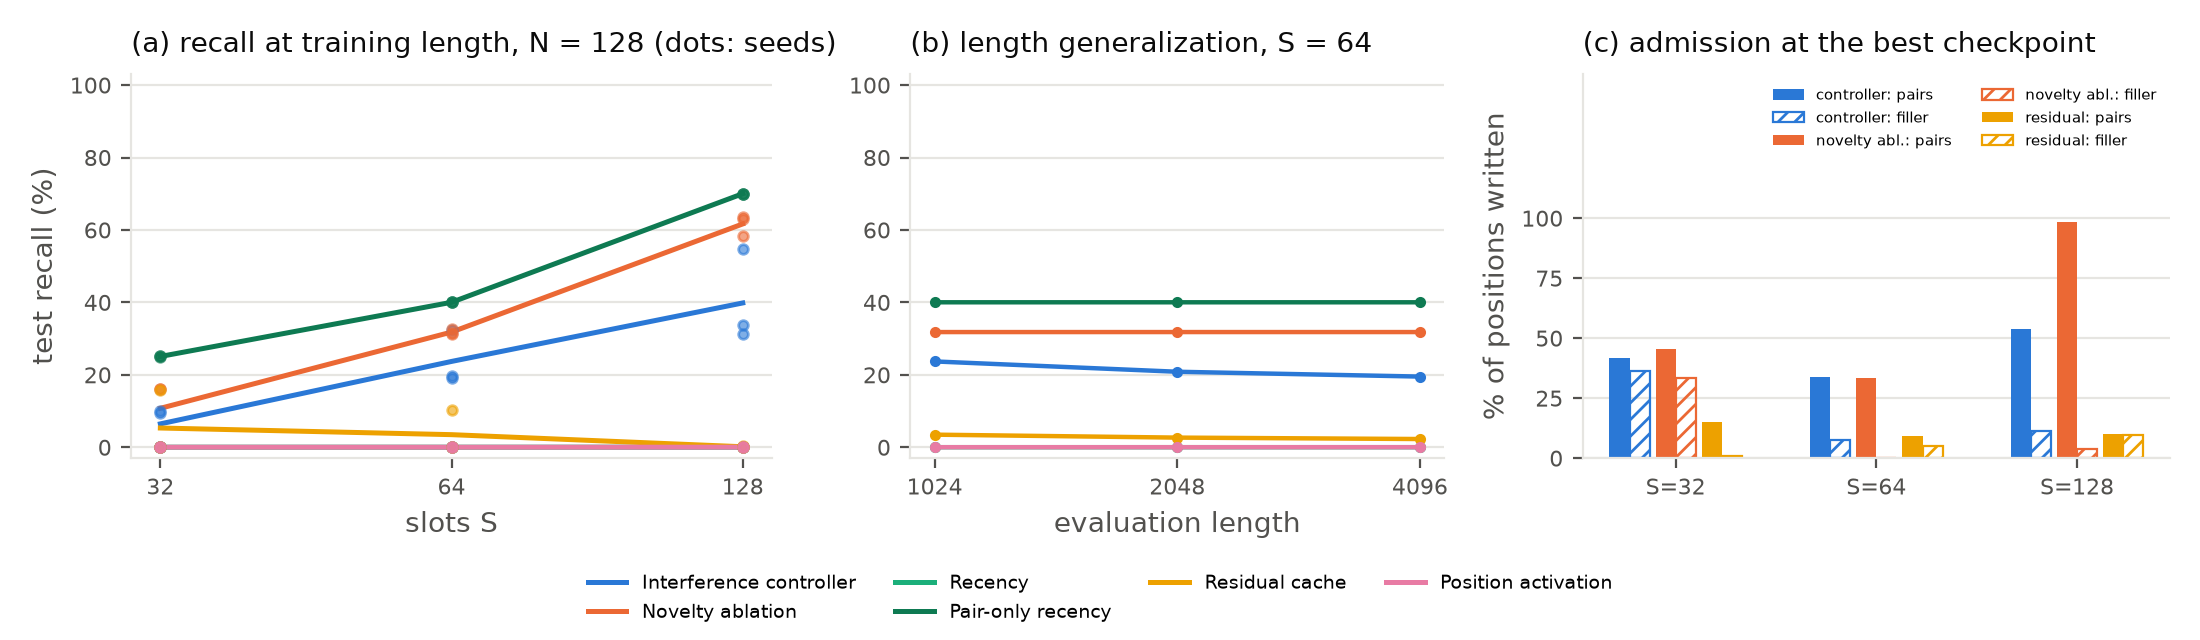
\includegraphics[width=\textwidth]{figures/sweep_n128.png}
\caption{The $N = 128$ column (training length 1024, tests at 1024, 2048 and
4096). Same ordering as at $N = 64$ in every cell. Pair-only recency sits at
its ceiling at $S = 32$ (25 vs 24\%), 3~pp under at $S = 64$ and 11~pp under
at $S = 128$, the same shortfalls as the matching pairs-per-slot cells at
$N = 64$. The controller is the only writer whose recall falls with evaluation
length.}
\label{fig:sweep128}
\end{figure*}

\textit{H1 test.} H1 is not supported at any budget at $N = 64$. The
strongest rule-based writer in every cell is pair-only recency, and it beats
the controller by 6.6~pp at $S = 64$ (per-seed $-5.8$ to $-7.4$), by 17~pp in
the capacity-bound $S = 32$ cell, and by 33~pp at $S = 128$, where it is
perfect and the controller averages 67\% with one seed at 48\%. The
admission statistics (Fig.~\ref{fig:sweep}c) give the mechanism: the learned
gate admits 69\% of pairs at $S = 64$ and 82\% at $S = 128$ while still
writing some filler, whereas the parameter-free rule admits every pair and
nothing else. At $S = 64$ a writer that admitted every pair could reach 81\%
(the ceiling of Section~\ref{sec:protocol}); the controller's shortfall is an
under-admission failure, not a capacity one. At $N = 128$ the ordering is the
same in every cell: $-19$, $-16$ and $-30$~pp at $S = 32$, 64 and 128, every
seed negative, with the controller bimodal across
seeds as before. Against the proposal's own baselines (recency, residual cache,
position activation), which are at or near chance in every cell above $S = 32$
except naive recency at 64 associations and 128 slots (29\%),
the controller wins by 20 to 63~pp over the best of them. That margin is a
finding in its own right, but it is not H1: H1 names the strongest
validation-selected baseline, and that baseline is the pair-only reference
added in Section~\ref{sec:protocol}, which no writer without the generator's
layout could implement exactly.

\textit{H2 test.} H2 is refuted. The decisive comparison is the input-only
ablation, whose gate sees nothing derived from the stored keys or values,
trained at the controller's learning rate: it scores 66.0\% at $S = 64$ (seeds
65.8 to 66.1) and 94.0\% at $S = 128$ (93.0 to 95.6), beating the controller by
2.5 and 27~pp with every seed positive, and matching the novelty ablation
within 0.2 and 2.0~pp. It has the tightest seed spread of any learned writer.
Its admission statistics show what it learned: 71 to 91\% of pairs and under
4\% of filler at $S = 64$, i.e.\ ``this token is a pair's value position'',
read off the backbone's content projection. Key novelty added on top of that
moves recall by at most 2~pp; the per-slot key similarity and value
disagreement make the gate admit fewer pairs and vary more across seeds. The best-of-each
comparison in the upper rows of Table~\ref{tab:final}, which had the controller
17.9~pp ahead of the novelty ablation at $S = 64$, is a learning-rate artefact:
the ablation's selected rate, $10^{-3}$, came from a single seed at $S = 32$,
and at that rate every learned writer writes every pair plus 18 to 23\% of
filler. At equal rates the ordering is input-only $\geq$ novelty ablation $>$
controller at both budgets, and inside the capacity-bound $S = 32$ cell the
novelty ablation is ahead of the controller by 4.8~pp on every seed. The
interference signal carries no information a learned admission gate can use on
this task; a gate that ignores memory entirely is within 2~pp of the best
learned writer at both budgets, and 4 to 6~pp under the parameter-free
reference.

\textit{Length generalization.} Fig.~\ref{fig:sweep}(b). (Test sets at
$2\times$ and $4\times$ the training length share keys, values and query
positions across writers but not filler tokens, which the generator draws from
the global RNG; comparisons at those lengths are paired on associations only.) Every writer with a
flat policy is flat in length (the fixed rules within 0.1~pp from 512 to 2048,
the learned ablations and the residual cache within 2~pp).
The controller loses 2.4~pp at $S = 64$ and 9~pp at $S = 128$, and naive
recency loses 8~pp at $S = 128$; both are writers whose gate statistics drift
with position.

\textit{Delay sweep.} Not run. The flat length curves above show why it is
the extrapolation test this protocol lacks: only a query gap that scales with
length would separate load from elapsed context, and it is left as future
work.

\textit{How each writer spends its budget.} Fig.~\ref{fig:sweep}(c), at the
best checkpoint, mean over seeds. The controller's write fraction rises with
budget (0.10, 0.13, 0.26 of positions at $S = 32$, 64, 128) and so does its
pair admission (29\%, 69\%, 82\%); filler admission is 6\%, 1\%, 13\%. The
ablation writes every pair from $S = 64$ up and 18--20\% of filler. The
residual cache's threshold separates pairs from filler only at $S = 32$ (69\%
vs 7\%); at 64 and 128 slots it admits 24--32\% of every class alike, which is
why it is at chance there (Table~\ref{tab:final}). Slot entropy is within 0.01
bits of its maximum for every learned writer at every budget, so no writer
collapses onto a subset of slots; the differences are in \emph{what} is
admitted, not \emph{where}.

\textit{Cost.} Every writer has 5.99M parameters; the learned writers add
5{,}715 to the rule-based ones (1{,}603 in the gate networks and 4{,}112 in the
content projection), the residual cache 2. State per sequence at $S = 64$ is
129~KB (64~KB backbone, 65~KB memory). On the compiled fast path at length 512
a run takes 13 to 19 minutes for the rule-based writers (230k to 330k tokens
per second) and 23 to 29 for the learned ones (150k to 190k), two sharing an
RTX 5090 at 12 to 16~GB each; at length 1024, 27 to 62 minutes, one at a time
at 18 to 30~GB. Test evaluation on 10{,}000 sequences takes 3 to 10~s at
length 512, 10 to 31~s at 1024, and up to 7.7 minutes at 4096. Training plus
test time sums to 56 GPU-hours for the 108 sweep runs, 15 for the 36 follow-up
runs at the target, and 7 for the 24 skew-pilot runs.

\textit{Hyperparameter selection.} Table~\ref{tab:hparams} gives the
validation recall of the best checkpoint at $N = 64$, $S = 32$, seed 0, for
each writer across the learning-rate grid $\{3\times10^{-4}, 6\times10^{-4},
10^{-3}\}$ (a probe at $10^{-4}$ never left chance within 8000 steps) and, for
the controller, hidden sizes $\{32, 64, 128\}$ at $3\times10^{-4}$. Selected:
controller $3\times10^{-4}$ with hidden size 32; the novelty ablation
$10^{-3}$ with hidden size 32 (it shares the controller's architecture and
differs only in the removed features); residual cache $6\times10^{-4}$; the
recency writers and position activation $3\times10^{-4}$ (the latter is at
chance at every learning rate because it writes at every position at this
density). Each cell is one seed, and the write policy a run settles into is
stochastic (the "Capacity ceiling" paragraph of Section~\ref{sec:protocol}), so neighbouring cells can differ by
more than the seed spread; the sweep's three seeds are the confirmation. The
hidden-size-32 controller is also the only controller run whose validation
recall rises monotonically to the end of the schedule. A post-sweep
re-selection of the controller at $N = 64$, $S = 64$ on three seeds (learning
rate $\{3, 6, 10\} \times 10^{-4}$, hidden size $\{32, 64\}$) confirms the
choice: $3 \times 10^{-4}$ with hidden size 32 averages 63.5\% validation
recall with all three seeds within 2~pp, and every other setting averages 40
to 44\% with two of three seeds in a poor basin.

\begin{table}[t]
\caption{Hyperparameter selection: validation recall (\%) of the best
checkpoint at $N = 64$, $S = 32$, seed 0. Bold marks the selected value.}
\label{tab:hparams}
\centering
\begin{tabular}{lccc}
\toprule
writer & lr $3\times10^{-4}$ & $6\times10^{-4}$ & $10^{-3}$ \\
\midrule
controller (hidden 64) & \textbf{19.0} & 20.9 & 17.6 \\
novelty ablation (hidden 64) & 19.4 & 19.0 & \textbf{27.7} \\
residual cache & 0.1 & \textbf{37.2} & 0.2 \\
pair-only recency & \textbf{40.1} & 40.1 & 40.0 \\
position activation & \textbf{0.0} & 0.0 & 0.0 \\
\midrule
controller hidden (lr $3\times10^{-4}$) & 32 & 64 & 128 \\
 & \textbf{32.5} & 19.0 & 24.6 \\
\bottomrule
\end{tabular}
\end{table}

\begin{table*}[t]
\caption{Pilot run, seed 0, 24 associations and 16 slots, trained at length
128. Exact recall (\%) on 10{,}000 test sequences with 95\% bootstrap CI; cost
columns measured on one RTX 5090.}
\label{tab:pilot}
\centering
\footnotesize
\begin{tabular}{@{}lrrrrrrrr@{}}
\toprule
Writer & Params & State/seq & Recall $L{=}128$ & Recall $L{=}256$ & Recall $L{=}512$ & Train (min) & Tok/s & GPU (MB) \\
\midrule
Interference controller & 2.84M & 80 KB & \textbf{51.9} [51.7, 52.2] & \textbf{52.1} [51.9, 52.3] & \textbf{52.1} [51.9, 52.3] & 16 & 34k & 871 \\
Novelty ablation & 2.84M & 80 KB & 50.7 [50.5, 50.9] & 50.8 [50.6, 51.0] & 50.9 [50.6, 51.1] & 15 & 36k & 806 \\
Recency & 2.84M & 80 KB & 11.0 [10.9, 11.1] & 9.6 [9.5, 9.7] & 8.7 [8.6, 8.8] & 7 & 78k & 590 \\
\bottomrule
\end{tabular}
\end{table*}

\begin{figure*}[t]
\centering
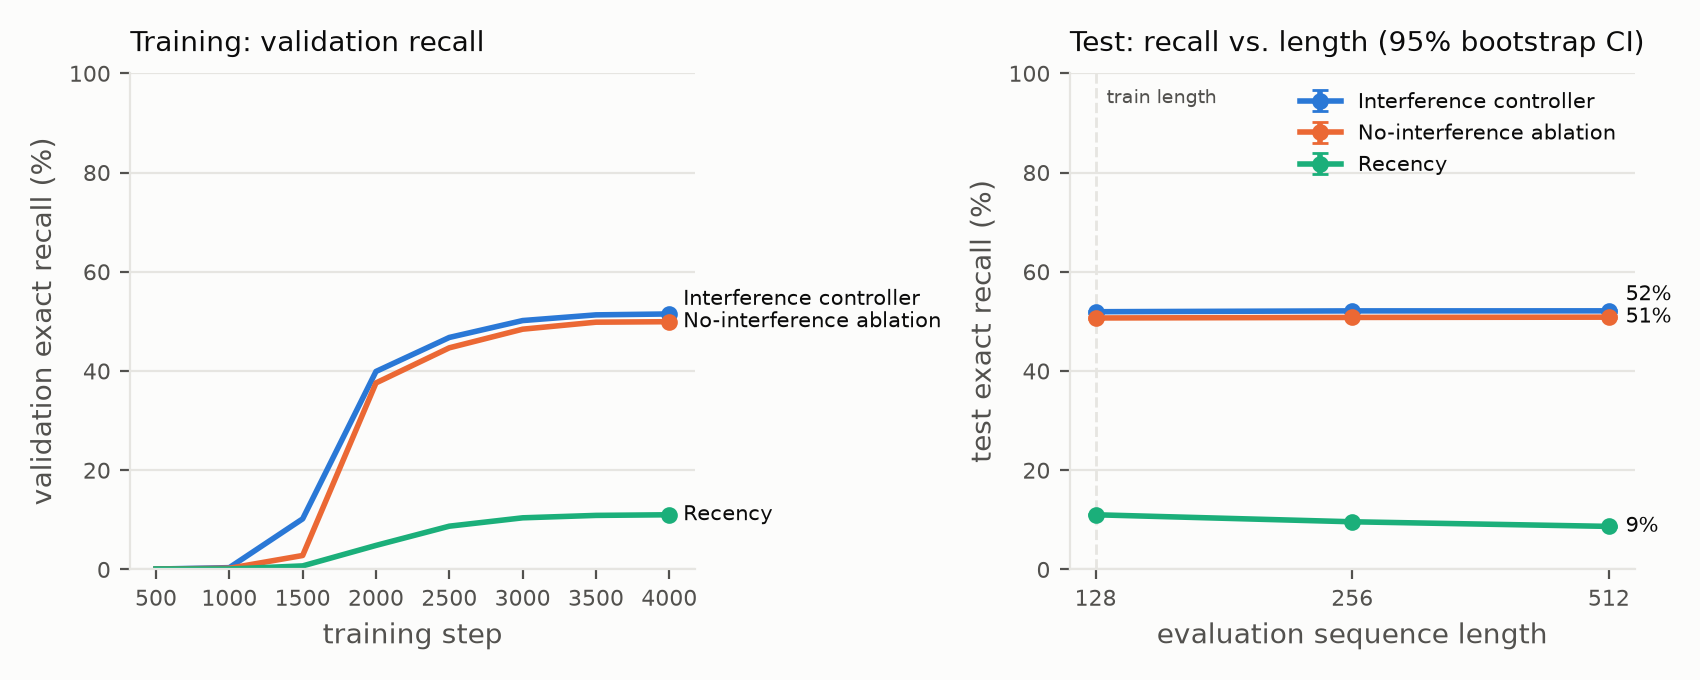
\includegraphics[width=0.9\textwidth]{figures/pilot.png}
\caption{Pilot run, seed 0. Left: validation exact recall during training.
Right: test recall against evaluation length (trained at 128), with 95\%
bootstrap intervals that are narrower than the markers.}
\label{fig:pilot}
\end{figure*}

\subsection{Pilot: pipeline validation}
\label{sec:pilot}

\textit{What the pilot is for.} A single seed, run to validate the pipeline end
to end, to find the task size at which learning happens within a short budget,
and to measure cost. The numbers below are one seed and carry no statistical
claim about H1 or H2.

\textit{The proposal's setting did not learn.} The first pilot used the
proposal's target: $N = 64$ with 16 updates and 16 distractors, 32 slots, length
512, vocabulary 8192, 8000 steps at batch 64. The recency baseline finished at
chance recall (0.01\%, where chance is 1/4096). The controller was at chance
after 2600 steps with the loss still at the unigram floor, and was stopped.
Diagnostics on smaller tasks then isolated three separate causes, fixed one at a
time with the smallest change that tested each hypothesis:

\begin{enumerate}
\item \textit{Key alignment.} Projecting the stored key from the value token's
position made the memory path useless until the backbone learned to copy keys
forward. The one-step shift of Section~\ref{sec:arch} took the recency writer
from 12\% to 47\% recall on an 8-pair task at equal steps.
\item \textit{Diffuse gates.} The soft sigmoid-times-softmax gate smeared each
write over all slots. The straight-through gate of Section~\ref{sec:controller}
took the controller from 11\% to 81\% on the same task.
\item \textit{Content-blind write decision.} With only memory statistics as
input, whether to write could not depend on what the token was, so storing
value tokens rather than filler was learned only when the backbone happened to
bootstrap it. Adding the 16-dimensional content projection took a 16-pair task
from 3\% to 92\% at 1400 steps, and a setting that the content-blind controller
never learned in 5000 steps started learning within 1400.
\end{enumerate}

After these fixes a one-factor scan from the smallest learnable task showed that
vocabulary (512 to 8192) and length (64 to 128) did not block learning, but the
ratio of associations to slots did, and the 64-association target was still at
chance after 1400 steps. The pilot therefore moved to the 24-association,
16-slot setting of Section~\ref{sec:task}. Reaching the proposal's target is the
first item of future work (Section~\ref{sec:changes}).

Two further problems appeared at that setting and were traced the same way:

\begin{enumerate}
\setcounter{enumi}{3}
\item \textit{Cold start.} With more associations than slots, the controller's
random initial policy thrashed the memory and the first 4000-step pilot stayed
at chance while recency reached 10.9\%. A learnable recency prior on the slot
logits (Section~\ref{sec:controller}) starts the controller as the recency
writer so retrieval works from step 0; in the diagnostic, recall then rose to
25\% by step 1000 instead of staying at chance.
\item \textit{Gradient blow-up in the memory loop.} Runs then collapsed after
about 1000 steps, and one produced a NaN loss. Per-group gradient norms showed
spikes of $10^4$ to $10^5$ in the writer, the projections, and the backbone
blocks, with the answer head unaffected, while the backbone trained alone never
exceeded 2. The source was the $1/\lVert x\rVert$ factor in the gradients of
the cosine similarity and the L2 disagreement: slot keys are convex mixtures
and can shrink toward zero. Adding an $\epsilon = 10^{-2}$ inside both square
roots bounded the gradient; the worst spike fell from 65{,}000 to 50 and the
collapse disappeared. Lowering the learning rate from $10^{-3}$ to $3 \times
10^{-4}$ on validation removed the remaining heavy clipping, and the pilot
backbone was reduced to two layers because depth only slowed learning at this
task size.
\end{enumerate}

\textit{Pilot numbers.} Table~\ref{tab:pilot} and Fig.~\ref{fig:pilot} give the pilot
numbers. Paired differences on the same 10{,}000 test sequences at $L = 128$:
controller minus recency $+40.9$~pp, paired 95\% CI $[+40.7, +41.2]$;
controller minus ablation $+1.3$~pp, paired 95\% CI $[+1.0, +1.5]$ (and the same
$+1.3$~pp at $L = 512$).

\textit{Pipeline checks that passed.} Unit tests cover split disjointness,
answer-position masking, the slot update's identity at zero gate, gate range and
normalization, and gradient flow into the controller and into both memory
projections. A 64-sequence overfit check drives the loss below 0.1 in 300 steps,
confirming that the read path can carry the answer.

\textit{Cost.} At this size one run was 16 minutes on an RTX 5090 at under
1~GB on the eager loop; the sweep's cost is given in Section~\ref{sec:final-results}.

%=====================================================================
\section{Discussion}
\label{sec:discussion}

\subsection{What the sweep shows}

Four things, each on three seeds per cell and paired on the same test
sequences.

\textit{The 32-slot cell cannot decide the hypotheses.} At 64 associations
with 16 updates and 16 distractors there are 96 pairs for 32 slots, and the
ideal online writer, which admits every pair, overwrites updates in place and
evicts the oldest, reaches 43\% (50\% with perfect distractor rejection). Every
writer in the study sits under that line, pair-only recency at 40\%, 3~pp
below the ideal, and the 7~pp between the online ceiling and the offline one,
the only margin allocation could win there, is narrower than the controller's
seed range in that cell (19 to 31\%). The proposal named this cell as the target. The ceiling was computed after
the first three-seed results there and moved the decisive cells to 64 and 128
slots; computed before the first target runs it would have saved a day of
probes into the post-peak drift of those runs, which the ceiling showed to be
a move into a worse write policy rather than a training failure.

\textit{A parameter-free rule beats every learned writer.} Pair-only recency
has no parameters in the writer and uses one fact about the task, which
positions hold pairs. It leads in all six cells, by 6.6~pp over the controller
at 64 associations and 64 slots and by 33~pp at 128 slots, where it is perfect,
and at 128 associations the margins are 16 to 30~pp (Table~\ref{tab:final}). The admission
statistics (Figs.~\ref{fig:sweep}c and~\ref{fig:sweep128}c) locate the loss:
the controller admits 69\% of pairs at 64 slots and 82\% at 128, and the rule
admits all of them. A writer that admitted every pair and rejected every
distractor could reach 100\% at 64 slots; no learned writer approached that,
and the best learned writer in each cell trails the rule by 4~pp (the
input-only ablation at 66.0\% at 64 slots; the novelty ablation at 96.0\% at
128). Against the proposal's own baselines the picture reverses: the
residual cache and position activation are at or near chance above 32 slots,
naive recency reaches 29\% only at 128 slots, and the controller beats the
best of the three by 20 to 63~pp in every such cell. H1 nevertheless fails as defined, because it is stated against the
strongest validation-selected baseline and that baseline is the reference
the proposal lacked; the margin over the proposal's own baselines is reported
as a separate result.

\textit{The interference signal carries nothing usable.} The decisive
comparison is the input-only ablation, whose gate sees the content projection
of the current token and the slots' age, usage, and occupancy, and nothing
derived from stored keys or values. At the controller's learning rate it beats
the controller by 2.5~pp at 64 slots and 27~pp at 128, every seed positive,
and matches the novelty ablation within 2~pp. Adding key novelty moves recall
by at most 2~pp; adding per-slot similarity and value disagreement makes the gate
admit fewer pairs and vary more across seeds (one of three controller seeds at
128 slots reached 48\% against 75 and 78). The gate that works learns one
thing, ``this token is the value position of a pair'', and reads it off the
backbone's representation of the token. The best-of-each comparison, which
had the controller 17.9~pp ahead of the novelty ablation at 64 slots, was a
learning-rate artefact of one-seed selection at the capacity-bound cell, and
the three-seed re-selection of the controller at the decisive cell returned
the sweep's own setting (63.5\% against 40 to 44\% for every other), so the
controller's loss is not a tuning accident.

\textit{Length does not matter; load does.} Every writer with a
position-independent policy is flat from the training length to four times
it, the fixed rules to within 0.1~pp and the learned ablations and the
residual cache to within 2~pp, because the task's context block is fixed and longer
sequences add only filler. The two writers that degrade with length, the
controller and naive recency, are the two whose admission drifts with
position; writing filler alone does not do it, since the novelty ablation at
its selected rate writes 18 to 20\% filler and is flat. This is the
memory-load account of Lee et al.~\cite{lee2026howlinear} seen from the
memory side: adding tokens that are not associations adds no load, and recall
does not move. The flat curves also mean this protocol is a weak test of
extrapolation; a delay sweep whose query gaps scale with length is the test
that would not be flat, and it was not run.

\subsection{The writer as an online cache}

\textit{The writer is an online cache.} The slot memory is a cache of $S$
entries; each incoming pair is an insertion request that must be accepted or
dropped before the next token arrives, with no look-ahead. In that vocabulary
pair-only recency is FIFO eviction behind a perfect admission filter, the
capacity ceiling of Section~\ref{sec:protocol} is Belady's offline
optimum~\cite{belady1966study}, and H1 asks whether a learned admission policy
can beat FIFO online. Sleator and Tarjan~\cite{sleator1985amortized} showed
that no deterministic online eviction rule is better than a factor of $S$
from the offline optimum in the worst case, and that LRU and FIFO meet that
bound; the sharper point for this task is that when future requests are
independent of the past, an online policy has nothing to condition on, and
the only margin left is admission: rejecting tokens that will never be
queried. In MQAR as generated here every queried key is drawn uniformly from
the key vocabulary and every distractor key from the same pool, so at write
time a distractor is indistinguishable from a pair that will be queried, and
an update is recognizable only by its key already being stored. The
parameter-free rule therefore sits at the online optimum up to update
handling, and the sweep measures how close a learned gate gets to it: the
novelty and input-only ablations at the controller's learning rate come within
4 to 6~pp at both budgets, and the interference features move the gate away
from it. Seen
this way the negative result is the expected one, and the study's
contribution is the measurement of the gap and of its cause, under-admission
of pairs, rather than the direction of the sign.

\textit{Where a learned writer could win.} The same theory says when
learning should pay: when something observable at write time predicts reuse.
The learned-caching literature is built on exactly that condition. Lykouris
and Vassilvitskii~\cite{lykouris2018competitive} give an eviction rule whose
competitive ratio falls with the error of a next-use predictor and never
exceeds the no-advice bound; Song et al.~\cite{song2020lrb} train a predictor
of Belady's decision from features of the request stream; and TinyLFU
\cite{einziger2017tinylfu} is a frequency-based admission filter in front of
a conventional eviction rule, which is structurally what our controller is.
All three assume a skewed, temporally correlated request stream. We tested
this condition directly at the pilot scale (24 associations, 16 slots, length
128, three seeds): queried keys drawn from a Zipf distribution with exponent 2
over the key vocabulary and distractor keys from its cold remainder, so that
the key embedding alone predicts whether a pair will be queried; the controller and
pair-only recency trained for 12{,}000 steps at both distributions, and the
novelty ablation at the skewed one.
The prediction from the caching view held on the admission side and failed on
recall. With the reuse signal the controller learned to reject distractors on
two of three seeds (distractor admission 0.50 and 0.24 against pair admission
0.91 and 0.90; the third seed never left write-everything), the novelty
ablation on one of three, and at the uniform distribution all three controller
seeds converged toward admitting every token, which is FIFO. But pair-only
recency gains from the skewed distribution too, 79.6\% against 76.4\% at the
uniform one on the same schedule (three seeds within 1~pp in each), because
the skew makes the read easier for every writer. Against that matched control
the controller trails by 7.6~pp at the uniform distribution and by 1.1~pp on
its two good seeds at the skewed one (78.5 against 79.6), with the third seed
17~pp behind. The learned rejection therefore closes most of the gap to the
non-learned rule where it is learned, and does not cross it. At this scale the
learned rejection buys nothing: FIFO loses about 2.4 of 16 slots to
distractors, and the controller gives up 10\% of pairs to reject half of them.
Two further points carry back to the sweep. The controller gained 18~pp from
4{,}000 to 12{,}000 steps at the pilot scale, so the 8{,}000-step schedule of
Table~\ref{tab:final} may under-train the learned writers, and the
basin-dependence seen there recurs here (one seed in three). A writer that
could turn the reuse signal into a recall gain would need to reject
distractors without under-admitting pairs, and the budget where that trade
pays is one where distractors cost more than a sixth of the slots.

\subsection{Comparison with the cited mechanisms}

Of the three mechanisms the baselines model, the input-dependent router
(Raven~\cite{afzal2026raven}, our novelty and input-only ablations) is the
strongest: at the controller's learning rate it reaches 66\% at 64 slots and
94 to 96\% at 128, within 4 to 6~pp of the reference. The residual-gated admission
of HOLA~\cite{cui2026hola} learned a useful threshold only at 32 slots, where
it averaged 30\% with every seed above chance, 7~pp above the controller; above that its
learning rate, selected at 32 slots, left it admitting a quarter to a third of
every token class and at chance. That is an under-tuned baseline, not a
refutation of HOLA, whose cache is exact and whose residual comes from a full
language model. Position scheduling (Proteus~\cite{bayat2026proteus}) has no
admission rule and writes at every position, so at this density it is a
recency variant and stays at zero; its contribution in the original is
capacity growth, which this protocol does not test. The gain the capacity
analyses predicted for an interference signal at high load, where the
proposal expected the controller to pull away, does not appear: at 128
associations the controller's deficit to the reference is 16 to 30~pp, and at
no budget or load does it come within 6~pp.

\subsection{Strengths and limitations}

\textit{Strengths.} The comparison is controlled: every writer shares the
backbone, projections, memory, answer head, data, schedule, and state budget,
and the two ablations change input features without changing a single
parameter. Test sequences at the training length are identical across
writers for a seed, so every number in Table~\ref{tab:final} is exactly
paired. Each batch of runs after the pilot was pre-registered with a prediction,
and the predictions that failed (the controller's hidden size, the equal-learning-rate
check, the skewed-key pilot) are reported as failures. The two checks that
changed the paper's claims, the equal-rate comparison and the input-only
ablation, were run because a stated concern and a code audit called for them,
and both are in the record.

\textit{Limitations.} Hyperparameters were selected on one seed per grid
point (Table~\ref{tab:hparams}), and the sweep shows the cost: the hidden size
chosen for the controller gave 32.5\% on its grid seed and 19, 19 and 31\% on
the three sweep seeds at the same setting, and the residual cache's learning rate,
chosen at $S = 32$ where it then learned on all three seeds, leaves it at
chance at 64 and 128 slots. The sweep's best-of-each H2 comparison would have
supported H2 at $S = 64$; only the equal-learning-rate check showed the gap
was the ablation's one-seed rate selection, and only a code audit showed that
the pre-registered ablation still saw key novelty, which is why the input-only
ablation was added after the sweep. The selection recipe, not the
sweep, is what one seed per grid point weakens. The learned writers
are bimodal across seeds (one of three controller seeds at $S = 128$ reached
48\% against 75 and 78), so the three-seed means carry a spread the pooled
bootstrap interval does not show. Re-selecting the controller's learning rate and hidden
size at $N = 64$, $S = 64$ on three seeds (six settings, 18 runs, 12 of them new) returns the
sweep's own setting as the best by 20~pp, so the H1 result at the decisive
cell holds under three-seed selection there, not only under the original
one-seed choice. The 8000-step schedule, fixed before the
sweep, may under-train the learned writers: several controller runs at
$S = 64$ and $S = 128$ were still rising at the last evaluation, and a pilot
on a skewed key distribution (Section~\ref{sec:discussion}) found that the
controller's gate only learned to separate hot from cold keys when given three
times the schedule. Any follow-up should match a longer schedule across
writers. Five design changes (key shift, straight-through gates,
content input, recency prior, $\epsilon$-safe features) were made after the
proposal and before any baseline-vs-controller comparison; they apply to all
writers, but they were motivated by getting the controller to learn, and the
baselines were tuned only through the learning-rate grid of
Table~\ref{tab:hparams}. The task is
synthetic: results bound what allocation can do on associative recall and do
not establish language-model gains. Finally, the memory update is a sequential
loop over tokens, which limits the scale the sweep can reach.

\subsection{What changed between the proposal and the final experiment}
\label{sec:changes}

Every change is dated in the project's lab notebook; the ones that affect
interpretation are:
\begin{enumerate}
\item \textbf{Target settings.} The proposal's 64-association, 32-slot target
did not learn with the pilot's four layers and learning rate $10^{-3}$; two
layers and $3 \times 10^{-4}$, found by one-variable probes, became the frozen
backbone setting; each writer's learning rate was then selected on validation
(Table~\ref{tab:hparams}). Vocabulary 8192, 8000 steps and weight decay 0.1 were
kept.
\item \textbf{Capacity ceiling and the pair-only reference.} After the first
three-seed results at the target, the ceiling simulation showed the cell was
capacity-bound; the pair-only recency writer was added as the non-learned
reference, naive recency was kept as a control, and the hypotheses were moved
to 64 and 128 slots. The $N = 128$ column trains at length 1024 because its
context block does not fit in 512.
\item \textbf{Checkpoint selection.} Test evaluations use the checkpoint with
the best validation recall rather than the last, because the cosine tail moved
several controller runs into a worse write policy after their peak.
\item \textbf{Equal-learning-rate check.} Twelve runs between the two sweep
columns, with
each learned writer at the other's rate, replaced the best-of-each H2
comparison as the reported one.
\item \textbf{Input-only ablation.} A code audit after the sweep found the
pre-registered ablation still saw key novelty; a second ablation with that
feature zeroed was added, pre-registered, and run on the same cells and seeds.
\item \textbf{Re-selection.} The controller's learning rate and hidden size
were re-selected at the decisive cell on three seeds after the sweep; the
sweep's setting won, so no cell was re-run.
\item \textbf{Speed.} The per-timestep memory update was compiled and the
whole step captured as a CUDA graph, numerically identical to the eager loop
and 3.4 times faster; without it the sweep would not have fit the schedule.
\end{enumerate}

%=====================================================================
\section{Conclusion}
\label{sec:conclusion}

This work asked whether a bounded memory beside a recurrent state should
decide what to store by looking at what is already stored. Under a protocol
fixed before the sweep, with 108 sweep runs on three seeds per cell and 60
follow-up runs, the answer on multi-query associative recall is no. A learned
controller with per-slot interference features loses to a parameter-free rule
that admits every key-value pair and nothing else, in every cell, by 6.6
points at the decisive budget and by 16 to 33 points elsewhere (H1 not
supported). The controller does beat the three baselines the proposal named,
by 20 to 63 points above 32 slots, but H1 is defined against the strongest
validation-selected baseline, and that is the rule. An ablation whose gate sees nothing from the
memory beats the controller at both decisive budgets and matches its best
ablation, so the interference signal adds no usable information (H2
refuted). The mechanism is measured, not inferred: learned gates under-admit
pairs; the per-slot interference features lower admission and widen the seed
spread, and key novelty moves recall by at most 2~pp.

Three things the study establishes beyond the hypotheses. The proposal's
target cell is capacity-bound: an ideal online writer caps at 43\% there, and
a ceiling simulation that costs seconds would have moved the target before any
training run. The pair-only rule is the bar: when queries are uniform over keys,
stored content cannot predict reuse, as the caching literature says, so the
only margin left to a learned policy is admission, and this rule, 3 to 11~pp
under the online ceiling, is the best policy tested; a learned admission
policy for bounded memories should be reported against it. And one-seed hyperparameter selection in a cell that
cannot separate policies produced a false positive for H2 that survived the
sweep and fell only to an equal-learning-rate check; the re-selection on three
seeds at the decisive cell is what supports stating the negative result.

What the study does not rule out. The learned writers trained for a fixed
8000 steps, and in the skewed-key pilot the controller gained 18~pp between
4{,}000 and 12{,}000 steps; a longer matched schedule could narrow the 4 to
6-point gap between the best learned writer and the rule, though at the pilot
scale it did not close it. The baselines are simplifications of the cited mechanisms,
re-implemented without public code, and the residual cache in particular was
under-tuned above 32 slots. The task is synthetic, and its queries are
uniform over keys, which is exactly the regime where stored content cannot
predict reuse; the skewed-key pilot is one step toward the regime where it
can, and there the gate did learn to reject distractors on two of three seeds
and still trailed the rule by 1~pp on those seeds and 6~pp on the three-seed
mean.

The direction the evidence supports is not a larger controller. It is an
admission module on a published cache, trained with a direct admission signal
rather than through a 512-step recurrence, and evaluated on request streams
with real reuse structure against the pair-only bar. On the task as posed, the best
write policy tested has no parameters.

\bibliographystyle{IEEEtran}
\bibliography{refs}

\end{document}
